\newpage
\section*{2\quad Tokens, and words as points in space}
\addcontentsline{toc}{section}{2 Tokens, and words as points in space}
\startchapter{2}

\begin{chaptermap}
A model cannot read. It receives numbers. This chapter answers two questions: how do we cut text into
pieces the model can count (\emph{tokens}), and how does each piece become an arrow of $d$ numbers
(an \emph{embedding})? We try whole words, then single letters, watch both break on real text, and arrive
at byte-pair encoding. Then we turn each token into an arrow, first by plain lookup and then by asking
where good arrows come from. It ends with Requirement 1 of Chapter 1 met: similar words sit near each
other, and Chapter 3 can start moving them.
\end{chaptermap}

\machine{2}{You are here: Chapter 2 builds the first two blocks, cutting text into tokens and looking up one arrow per token. Every later block works on these arrows.}

\begin{beforeyoustart}
(1) In a list of 1000 words, 25 have never been seen before. What percentage is that?
(2) Count the pairs of letters in the word \tok{banana}, reading left to right. How many times does
\tok{an} appear? (3) A table has 12 rows and 4 columns. How many numbers does it hold?
(4) If two arrows point at right angles, what is their dot product?

\smallskip\noindent\textit{Refreshers.} (1) $25/1000 = 0.025$, which is 2.5\%. (2) The pairs are \tok{ba},
\tok{an}, \tok{na}, \tok{an}, \tok{na}: \tok{an} appears twice. Overlapping pairs count separately.
(3) $12\times4=48$. (4) Zero (Chapter 3, \S3.2): no shadow, nothing in common.
\end{beforeyoustart}

%---------------------------------------------------------------------
\subsection*{2.1\quad What does the model receive?}

\Predict When you type \tok{waste of time} into a chat model, what arrives at the first layer of the
model: letters, words, or something else? Write your guess down before reading on.

The answer is a short list of whole numbers, one per piece of text, such as $(\nTwoTimeId)$ for the
toy word \tok{time}. Everything the model will ever know about your message has to travel through those
numbers. So the first design decision in any language model is a quiet one: \emph{what counts as one
piece?} Let us try the two obvious answers and watch them break, with numbers from the same corpus as
Chapter 1: transcribed technical talks on AI engineering, split into nine parts.

\Summary{the model never sees text, only a list of token numbers, so we must decide what one token is.}

%---------------------------------------------------------------------
\subsection*{2.2\quad Two simple choices, and how each breaks}

\paragraph{Choice 1: one token per word.} This is how you read, so it feels natural. In parts 1--8 there
are \cTrainWords\ words but only \nTwoWordVocab\ different ones, so the table of words is small.

\paragraph{How it breaks.} Language keeps inventing words. In part 9, \nTwoUnseenWordPct\% of the
words (\nTwoUnseenTypes\ different ones) never appeared in parts 1--8, and a word-level model has no
row for any of them. What would you do with a word you have no row for? Use the nearest known word? Split it
into smaller pieces? Write it down as ``unknown''? All three are reasonable guesses.

Older systems did the last one: every new word became one special token, \tok{<unk>}, and all of them
looked the same to the model. A customer who writes a product name the model has never seen would be
answered as if they had written nothing. And the long tail is not small: \nTwoSingletonPct\% of the
different words in parts 1--8 (\nTwoSingletons\ of them) appear exactly once.

\paragraph{Choice 2: one token per letter.} There are only \nTwoChars\ different letters in the
corpus, so nothing is ever unknown.

\paragraph{How it breaks.} The text gets long. An average word here is \nTwoCharsPerWord\ letters, plus a
marker for the end of the word, about \nTwoTpwZero\ tokens per word. Chapter 3 compares every token with
every earlier token, so the work grows with the \emph{square} of the length: roughly $\nTwoTpwZero^2
\approx \nTwoPairFactor$ times more comparisons than one token per word. And a single letter carries
almost no meaning, so the model must spend layers re-assembling words before it can think about them.

\begin{checkq}
You are building a model for a support team whose customers often type new product names. Which choice
breaks for them first, and why?
\begin{options}
\item One token per word, because every new product name has no row in the table.
\item One token per letter, because product names are long.
\item Neither, because the model reads the name the way a person does.
\item One token per word, because product names are longer than other words.
\end{options}
\end{checkq}

\Summary{whole words leave new words with nowhere to go; single letters make every sentence about five
times longer and attention about \nTwoPairFactor\ times more expensive.}

%---------------------------------------------------------------------
\subsection*{2.3\quad The middle path: byte-pair encoding}

\Predict Suppose you could give a few hundred common letter-groups their own token, and spell everything
else out of letters. Which groups would you pick first?

\Picture Think about how people take fast notes. Nobody invents a shorthand for a word used once, but a
phrase you write twenty times in a meeting soon gets an abbreviation. Byte-pair encoding does exactly
that, automatically: it looks for the pair of symbols that sits side by side most often in the text, and
gives that pair its own symbol. Then it does it again, and again.

\paragraph{The numbers.} We ran it from scratch on parts 1--8 (the script is \texttt{code/ch2\_bpe.py}).
Each word starts as its letters followed by an end-of-word marker \tok{\_}, so the word \tok{time}
starts as \nTwoSegZeroTime. The first merges, with how often each pair appeared:

\begin{center}
\small
\begin{tabular}{@{}r l r@{\qquad}r l r@{}}
\toprule
merge & pair & times seen & merge & pair & times seen\\
\midrule
1 & \nTwoMergeOne & \nTwoMergeCountOne & 5 & \nTwoMergeFive & \nTwoMergeCountFive\\
2 & \nTwoMergeTwo & \nTwoMergeCountTwo & 6 & \nTwoMergeSix & \nTwoMergeCountSix\\
3 & \nTwoMergeThree & \nTwoMergeCountThree & 7 & \nTwoMergeSeven & \nTwoMergeCountSeven\\
4 & \nTwoMergeFour & \nTwoMergeCountFour & 8 & \nTwoMergeEight & \nTwoMergeCountEight\\
\bottomrule
\end{tabular}
\end{center}

\noindent Did your prediction include \tok{e\_}, a word ending in ``e''? Very few people guess it, and it
is the most common pair of all. After \nTwoMerges\ merges the vocabulary has \nTwoBpeVocab\ symbols, and
our running words split like this:

\begin{center}
\small
\begin{tabular}{@{}l l l l@{}}
\toprule
word & 0 merges & 100 merges & \nTwoMerges\ merges\\
\midrule
\tok{waste} & \nTwoSegZeroWaste & \nTwoSegHundredWaste & \nTwoSegWaste\\
\tok{of} & \nTwoSegZeroOf & \nTwoSegHundredOf & \nTwoSegOf\\
\tok{time} & \nTwoSegZeroTime & \nTwoSegHundredTime & \nTwoSegTime\\
\bottomrule
\end{tabular}
\end{center}

Common words become one token. Rarer words become a few familiar pieces. And now the real test: the word
\tok{\nTwoUnseenWord} appears \nTwoUnseenWordCount\ times in part 9 and never in parts 1--8. A
word-level model would have nothing. Byte-pair encoding writes it as \nTwoSegUnseen. Of the
\nTwoTestWords\ words in part 9, the number that cannot be written at all is \nTwoUnkAfter, and the
average word costs \nTwoTokPerWord\ tokens, against \nTwoTpwZero\ for single letters.

\begin{figure}[h]
\centering
\begin{tikzpicture}
\begin{axis}[width=8.5cm, height=4.6cm, xlabel={vocabulary size (symbols)}, ylabel={tokens per word},
  xlabel style={font=\small}, ylabel style={font=\small}, tick label style={font=\small},
  axis lines*=left, mark size=1.6pt, ymin=1, ymax=5.6,
  nodes near coords, point meta=explicit symbolic, nodes near coords style={font=\footnotesize, anchor=south west}]
\addplot[black, mark=*] table[x=vocab, y=tpw, meta=merges] {data_ch2/bpe_growth.dat};
\end{axis}
\end{tikzpicture}
\caption{Measured on part 9: the more merges (numbers on the points), the fewer tokens each word costs.
The curve flattens, so the vocabulary size is a trade-off between table size and sequence length.}
\end{figure}

\Exactly Byte-pair encoding (Gage, 1994, as a compression method; Sennrich, Haddow and Birch, 2016, for
translation) builds the vocabulary in a loop:
\begin{enumerate}[label=\arabic*.]
\item Start with every word written as single symbols plus an end marker. The vocabulary is the set of
single symbols.
\item Count every pair of neighbouring symbols across the whole text, weighted by how often each word appears.
\item Add the most frequent pair to the vocabulary as one new symbol, and rewrite the text with it.
\item Repeat until the vocabulary has the size you chose.
\end{enumerate}
To cut new text into tokens, apply the learned merges in the order they were learned. GPT-2 (Radford
and colleagues, 2019) starts from the 256 possible \emph{bytes} instead of letters, so any text in any
language, including emoji and code, can always be written. Real tokenizers are this same loop run on far
more text: Qwen3 uses a vocabulary of 151{,}936 entries, as published in the Qwen3 technical report (2025;
we will check this against the model's \texttt{config.json} in Chapter 10). The tokenizer's own list
is slightly shorter, 151{,}669 entries; the embedding table is padded to a slightly larger size.

\begin{breaks}
Shorthand notes are written by one person for a reason they understand. Byte-pair encoding has no idea
what a pair means; it only counts. So \tok{e\_} becomes a token because it is frequent, not because it is a
unit of meaning. The model has to learn meaning later.
\end{breaks}

\Why Two pressures pull in opposite directions: a small vocabulary keeps the table small and leaves no word
unknown; a large vocabulary keeps sequences short. Frequency is a fair referee between them, because the
things you write often are the things worth a dedicated symbol.

\begin{wrongidea}{2.2}
``A word the model has never seen makes it fail or print \emph{unknown}.'' With byte-pair encoding there is
always a way to spell the word, down to single letters or bytes. The model never fails to \emph{read} a new
word. Whether it \emph{understands} it is a separate question: \tok{\nTwoUnseenWord} arrives as pieces, and
the model has to build the meaning from \tok{ok}, \tok{en}, \tok{iz}, \tok{er\_} and the words around them.
\end{wrongidea}

\begin{wrongidea}{2.3}
``A token is a word.'' It is tempting because for common words like \tok{of} and \tok{time} it is
true. But \tok{waste} became three tokens in our tokenizer. Measured on part 9, one of our tokens is on average \nTwoWordsPerTok\ of a word, and a rare word is
several tokens.
\end{wrongidea}

\begin{checkq}
After \nTwoMerges\ merges, \tok{time} is one token but \tok{waste} is three. What best explains this?
\begin{options}
\item \tok{time} is more important for meaning than \tok{waste}.
\item In parts 1--8, the pieces of \tok{time} were merged often enough to become one symbol, and
\tok{waste} was rarer.
\item The tokenizer splits every word into its syllables.
\item \tok{waste} has more letters, and long words are always split.
\end{options}
\end{checkq}

\Summary{byte-pair encoding gives frequent letter-groups their own token and spells everything else from
smaller pieces, so nothing is ever unknown and common words stay short.}

%---------------------------------------------------------------------
\subsection*{2.4\quad From a token number to an arrow: the embedding table}

\Predict The token \tok{time} is number \nTwoTimeId\ in our toy vocabulary and \tok{of} is number 1. Does
that mean \tok{time} and \tok{of} are similar, because 1 and \nTwoTimeId\ are close?

\Picture A token number is a locker number. Locker 2 is next to locker 1, but that tells you nothing
about what is inside. To get the contents you walk to the locker and open it. The embedding table is the
row of lockers, and each locker holds an arrow of $d$ numbers.

\paragraph{The numbers.} Our toy model knows \nTwoVocabSize\ tokens, each with an arrow of $d=4$ numbers.
First, the text becomes token numbers, one per token; a batch of sentences becomes a table of numbers:
\begin{center}% AUTO-GENERATED by code/figlib.py helpers -- do not edit
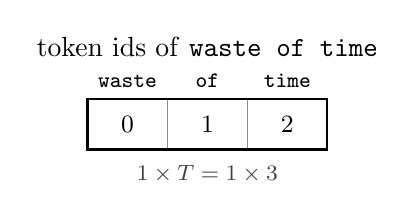
\begin{tikzpicture}[x=1.3cm]
\draw[black!45, fill=white] (0.000,0.000) rectangle (0.780,-0.640);
\node[font=\small, text=black] at (0.390,-0.320) {$0$};
\draw[black!45, fill=white] (0.780,0.000) rectangle (1.560,-0.640);
\node[font=\small, text=black] at (1.170,-0.320) {$1$};
\draw[black!45, fill=white] (1.560,0.000) rectangle (2.340,-0.640);
\node[font=\small, text=black] at (1.950,-0.320) {$2$};
\draw[line width=0.9pt] (0.000,0.000) rectangle (2.340,-0.640);
\node[anchor=south, font=\footnotesize\ttfamily] at (0.390,0.020) {waste};
\node[anchor=south, font=\footnotesize\ttfamily] at (1.170,0.020) {of};
\node[anchor=south, font=\footnotesize\ttfamily] at (1.950,0.020) {time};
\node[anchor=south, font=\normalsize] at (1.170,0.420) {token ids of \texttt{waste of time}};
\node[anchor=north, font=\footnotesize, text=black!75] at (1.170,-0.720) {$1\times T=1\times3$};
\end{tikzpicture}
\qquad\qquad
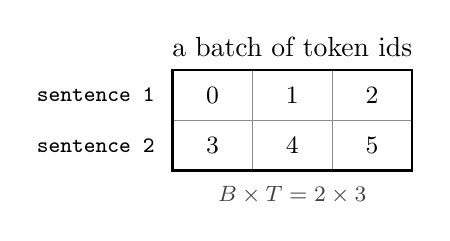
\begin{tikzpicture}[x=1.3cm]
\draw[black!45, fill=white] (0.000,0.000) rectangle (0.780,-0.640);
\node[font=\small, text=black] at (0.390,-0.320) {$0$};
\draw[black!45, fill=white] (0.780,0.000) rectangle (1.560,-0.640);
\node[font=\small, text=black] at (1.170,-0.320) {$1$};
\draw[black!45, fill=white] (1.560,0.000) rectangle (2.340,-0.640);
\node[font=\small, text=black] at (1.950,-0.320) {$2$};
\draw[black!45, fill=white] (0.000,-0.640) rectangle (0.780,-1.279);
\node[font=\small, text=black] at (0.390,-0.959) {$3$};
\draw[black!45, fill=white] (0.780,-0.640) rectangle (1.560,-1.279);
\node[font=\small, text=black] at (1.170,-0.959) {$4$};
\draw[black!45, fill=white] (1.560,-0.640) rectangle (2.340,-1.279);
\node[font=\small, text=black] at (1.950,-0.959) {$5$};
\draw[line width=0.9pt] (0.000,0.000) rectangle (2.340,-1.279);
\node[anchor=east, font=\footnotesize\ttfamily] at (-0.080,-0.320) {sentence 1};
\node[anchor=east, font=\footnotesize\ttfamily] at (-0.080,-0.959) {sentence 2};
\node[anchor=south, font=\normalsize] at (1.170,0.050) {a batch of token ids};
\node[anchor=north, font=\footnotesize, text=black!75] at (1.170,-1.359) {$B\times T=2\times3$};
\end{tikzpicture}
\end{center}
Each number opens one row of the embedding table $E$. Rows 0--2 are the arrows Chapter 3 uses; the
highlighted row is \tok{time}:
\begin{center}% AUTO-GENERATED by code/figlib.py helpers -- do not edit
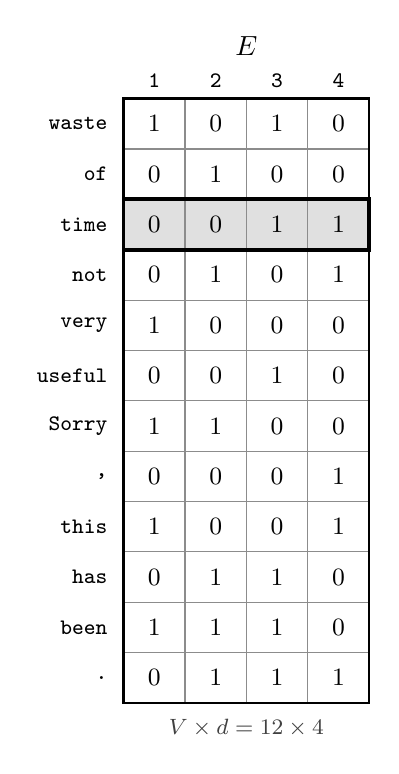
\begin{tikzpicture}
\draw[black!45, fill=white] (0.000,0.000) rectangle (0.780,-0.640);
\node[font=\small, text=black] at (0.390,-0.320) {$1$};
\draw[black!45, fill=white] (0.780,0.000) rectangle (1.560,-0.640);
\node[font=\small, text=black] at (1.170,-0.320) {$0$};
\draw[black!45, fill=white] (1.560,0.000) rectangle (2.340,-0.640);
\node[font=\small, text=black] at (1.950,-0.320) {$1$};
\draw[black!45, fill=white] (2.340,0.000) rectangle (3.120,-0.640);
\node[font=\small, text=black] at (2.730,-0.320) {$0$};
\draw[black!45, fill=white] (0.000,-0.640) rectangle (0.780,-1.279);
\node[font=\small, text=black] at (0.390,-0.959) {$0$};
\draw[black!45, fill=white] (0.780,-0.640) rectangle (1.560,-1.279);
\node[font=\small, text=black] at (1.170,-0.959) {$1$};
\draw[black!45, fill=white] (1.560,-0.640) rectangle (2.340,-1.279);
\node[font=\small, text=black] at (1.950,-0.959) {$0$};
\draw[black!45, fill=white] (2.340,-0.640) rectangle (3.120,-1.279);
\node[font=\small, text=black] at (2.730,-0.959) {$0$};
\draw[black!45, fill=black!12] (0.000,-1.279) rectangle (0.780,-1.919);
\node[font=\small, text=black] at (0.390,-1.599) {$0$};
\draw[black!45, fill=black!12] (0.780,-1.279) rectangle (1.560,-1.919);
\node[font=\small, text=black] at (1.170,-1.599) {$0$};
\draw[black!45, fill=black!12] (1.560,-1.279) rectangle (2.340,-1.919);
\node[font=\small, text=black] at (1.950,-1.599) {$1$};
\draw[black!45, fill=black!12] (2.340,-1.279) rectangle (3.120,-1.919);
\node[font=\small, text=black] at (2.730,-1.599) {$1$};
\draw[black!45, fill=white] (0.000,-1.919) rectangle (0.780,-2.558);
\node[font=\small, text=black] at (0.390,-2.239) {$0$};
\draw[black!45, fill=white] (0.780,-1.919) rectangle (1.560,-2.558);
\node[font=\small, text=black] at (1.170,-2.239) {$1$};
\draw[black!45, fill=white] (1.560,-1.919) rectangle (2.340,-2.558);
\node[font=\small, text=black] at (1.950,-2.239) {$0$};
\draw[black!45, fill=white] (2.340,-1.919) rectangle (3.120,-2.558);
\node[font=\small, text=black] at (2.730,-2.239) {$1$};
\draw[black!45, fill=white] (0.000,-2.558) rectangle (0.780,-3.198);
\node[font=\small, text=black] at (0.390,-2.878) {$1$};
\draw[black!45, fill=white] (0.780,-2.558) rectangle (1.560,-3.198);
\node[font=\small, text=black] at (1.170,-2.878) {$0$};
\draw[black!45, fill=white] (1.560,-2.558) rectangle (2.340,-3.198);
\node[font=\small, text=black] at (1.950,-2.878) {$0$};
\draw[black!45, fill=white] (2.340,-2.558) rectangle (3.120,-3.198);
\node[font=\small, text=black] at (2.730,-2.878) {$0$};
\draw[black!45, fill=white] (0.000,-3.198) rectangle (0.780,-3.838);
\node[font=\small, text=black] at (0.390,-3.518) {$0$};
\draw[black!45, fill=white] (0.780,-3.198) rectangle (1.560,-3.838);
\node[font=\small, text=black] at (1.170,-3.518) {$0$};
\draw[black!45, fill=white] (1.560,-3.198) rectangle (2.340,-3.838);
\node[font=\small, text=black] at (1.950,-3.518) {$1$};
\draw[black!45, fill=white] (2.340,-3.198) rectangle (3.120,-3.838);
\node[font=\small, text=black] at (2.730,-3.518) {$0$};
\draw[black!45, fill=white] (0.000,-3.838) rectangle (0.780,-4.477);
\node[font=\small, text=black] at (0.390,-4.157) {$1$};
\draw[black!45, fill=white] (0.780,-3.838) rectangle (1.560,-4.477);
\node[font=\small, text=black] at (1.170,-4.157) {$1$};
\draw[black!45, fill=white] (1.560,-3.838) rectangle (2.340,-4.477);
\node[font=\small, text=black] at (1.950,-4.157) {$0$};
\draw[black!45, fill=white] (2.340,-3.838) rectangle (3.120,-4.477);
\node[font=\small, text=black] at (2.730,-4.157) {$0$};
\draw[black!45, fill=white] (0.000,-4.477) rectangle (0.780,-5.117);
\node[font=\small, text=black] at (0.390,-4.797) {$0$};
\draw[black!45, fill=white] (0.780,-4.477) rectangle (1.560,-5.117);
\node[font=\small, text=black] at (1.170,-4.797) {$0$};
\draw[black!45, fill=white] (1.560,-4.477) rectangle (2.340,-5.117);
\node[font=\small, text=black] at (1.950,-4.797) {$0$};
\draw[black!45, fill=white] (2.340,-4.477) rectangle (3.120,-5.117);
\node[font=\small, text=black] at (2.730,-4.797) {$1$};
\draw[black!45, fill=white] (0.000,-5.117) rectangle (0.780,-5.756);
\node[font=\small, text=black] at (0.390,-5.437) {$1$};
\draw[black!45, fill=white] (0.780,-5.117) rectangle (1.560,-5.756);
\node[font=\small, text=black] at (1.170,-5.437) {$0$};
\draw[black!45, fill=white] (1.560,-5.117) rectangle (2.340,-5.756);
\node[font=\small, text=black] at (1.950,-5.437) {$0$};
\draw[black!45, fill=white] (2.340,-5.117) rectangle (3.120,-5.756);
\node[font=\small, text=black] at (2.730,-5.437) {$1$};
\draw[black!45, fill=white] (0.000,-5.756) rectangle (0.780,-6.396);
\node[font=\small, text=black] at (0.390,-6.076) {$0$};
\draw[black!45, fill=white] (0.780,-5.756) rectangle (1.560,-6.396);
\node[font=\small, text=black] at (1.170,-6.076) {$1$};
\draw[black!45, fill=white] (1.560,-5.756) rectangle (2.340,-6.396);
\node[font=\small, text=black] at (1.950,-6.076) {$1$};
\draw[black!45, fill=white] (2.340,-5.756) rectangle (3.120,-6.396);
\node[font=\small, text=black] at (2.730,-6.076) {$0$};
\draw[black!45, fill=white] (0.000,-6.396) rectangle (0.780,-7.036);
\node[font=\small, text=black] at (0.390,-6.716) {$1$};
\draw[black!45, fill=white] (0.780,-6.396) rectangle (1.560,-7.036);
\node[font=\small, text=black] at (1.170,-6.716) {$1$};
\draw[black!45, fill=white] (1.560,-6.396) rectangle (2.340,-7.036);
\node[font=\small, text=black] at (1.950,-6.716) {$1$};
\draw[black!45, fill=white] (2.340,-6.396) rectangle (3.120,-7.036);
\node[font=\small, text=black] at (2.730,-6.716) {$0$};
\draw[black!45, fill=white] (0.000,-7.036) rectangle (0.780,-7.675);
\node[font=\small, text=black] at (0.390,-7.355) {$0$};
\draw[black!45, fill=white] (0.780,-7.036) rectangle (1.560,-7.675);
\node[font=\small, text=black] at (1.170,-7.355) {$1$};
\draw[black!45, fill=white] (1.560,-7.036) rectangle (2.340,-7.675);
\node[font=\small, text=black] at (1.950,-7.355) {$1$};
\draw[black!45, fill=white] (2.340,-7.036) rectangle (3.120,-7.675);
\node[font=\small, text=black] at (2.730,-7.355) {$1$};
\draw[line width=1.4pt] (0.000,-1.279) rectangle (3.120,-1.919);
\draw[line width=0.9pt] (0.000,0.000) rectangle (3.120,-7.675);
\node[anchor=east, font=\footnotesize\ttfamily] at (-0.080,-0.320) {waste};
\node[anchor=east, font=\footnotesize\ttfamily] at (-0.080,-0.959) {of};
\node[anchor=east, font=\footnotesize\ttfamily] at (-0.080,-1.599) {time};
\node[anchor=east, font=\footnotesize\ttfamily] at (-0.080,-2.239) {not};
\node[anchor=east, font=\footnotesize\ttfamily] at (-0.080,-2.878) {very};
\node[anchor=east, font=\footnotesize\ttfamily] at (-0.080,-3.518) {useful};
\node[anchor=east, font=\footnotesize\ttfamily] at (-0.080,-4.157) {Sorry};
\node[anchor=east, font=\footnotesize\ttfamily] at (-0.080,-4.797) {,};
\node[anchor=east, font=\footnotesize\ttfamily] at (-0.080,-5.437) {this};
\node[anchor=east, font=\footnotesize\ttfamily] at (-0.080,-6.076) {has};
\node[anchor=east, font=\footnotesize\ttfamily] at (-0.080,-6.716) {been};
\node[anchor=east, font=\footnotesize\ttfamily] at (-0.080,-7.355) {.};
\node[anchor=south, font=\footnotesize\ttfamily] at (0.390,0.020) {1};
\node[anchor=south, font=\footnotesize\ttfamily] at (1.170,0.020) {2};
\node[anchor=south, font=\footnotesize\ttfamily] at (1.950,0.020) {3};
\node[anchor=south, font=\footnotesize\ttfamily] at (2.730,0.020) {4};
\node[anchor=south, font=\normalsize] at (1.560,0.420) {$E$};
\node[anchor=north, font=\footnotesize, text=black!75] at (1.560,-7.755) {$V\times d=12\times4$};
\end{tikzpicture}
\end{center}
To fetch \tok{time} with a multiplication, write its number as a \emph{one-hot} row: twelve zeros with a
single 1 in position \nTwoTimeId\ (counting from 0). Multiplying that row by $E$ picks out exactly one row,
because every other row is multiplied by 0:
\begin{figure}[!htb]\centering
\resizebox{\linewidth}{!}{% AUTO-GENERATED by code/figlib.py helpers -- do not edit
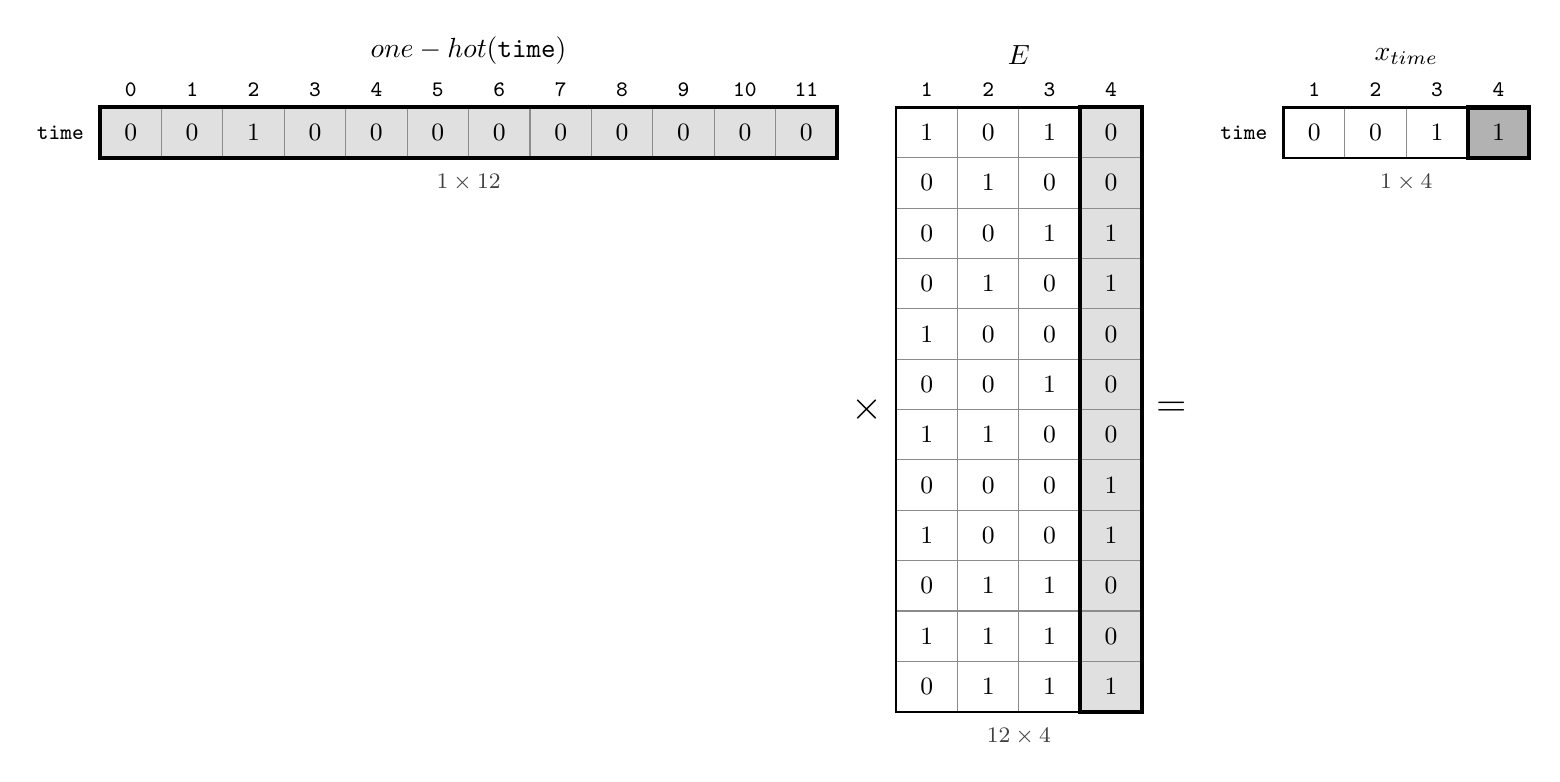
\begin{tikzpicture}
\draw[black!45, fill=black!12] (0.000,0.000) rectangle (0.780,-0.640);
\node[font=\small, text=black] at (0.390,-0.320) {$0$};
\draw[black!45, fill=black!12] (0.780,0.000) rectangle (1.560,-0.640);
\node[font=\small, text=black] at (1.170,-0.320) {$0$};
\draw[black!45, fill=black!12] (1.560,0.000) rectangle (2.340,-0.640);
\node[font=\small, text=black] at (1.950,-0.320) {$1$};
\draw[black!45, fill=black!12] (2.340,0.000) rectangle (3.120,-0.640);
\node[font=\small, text=black] at (2.730,-0.320) {$0$};
\draw[black!45, fill=black!12] (3.120,0.000) rectangle (3.900,-0.640);
\node[font=\small, text=black] at (3.510,-0.320) {$0$};
\draw[black!45, fill=black!12] (3.900,0.000) rectangle (4.680,-0.640);
\node[font=\small, text=black] at (4.290,-0.320) {$0$};
\draw[black!45, fill=black!12] (4.680,0.000) rectangle (5.460,-0.640);
\node[font=\small, text=black] at (5.070,-0.320) {$0$};
\draw[black!45, fill=black!12] (5.460,0.000) rectangle (6.240,-0.640);
\node[font=\small, text=black] at (5.850,-0.320) {$0$};
\draw[black!45, fill=black!12] (6.240,0.000) rectangle (7.020,-0.640);
\node[font=\small, text=black] at (6.630,-0.320) {$0$};
\draw[black!45, fill=black!12] (7.020,0.000) rectangle (7.800,-0.640);
\node[font=\small, text=black] at (7.410,-0.320) {$0$};
\draw[black!45, fill=black!12] (7.800,0.000) rectangle (8.580,-0.640);
\node[font=\small, text=black] at (8.190,-0.320) {$0$};
\draw[black!45, fill=black!12] (8.580,0.000) rectangle (9.360,-0.640);
\node[font=\small, text=black] at (8.970,-0.320) {$0$};
\draw[line width=1.4pt] (0.000,0.000) rectangle (9.360,-0.640);
\draw[line width=0.9pt] (0.000,0.000) rectangle (9.360,-0.640);
\node[anchor=east, font=\footnotesize\ttfamily] at (-0.080,-0.320) {time};
\node[anchor=south, font=\footnotesize\ttfamily] at (0.390,0.020) {0};
\node[anchor=south, font=\footnotesize\ttfamily] at (1.170,0.020) {1};
\node[anchor=south, font=\footnotesize\ttfamily] at (1.950,0.020) {2};
\node[anchor=south, font=\footnotesize\ttfamily] at (2.730,0.020) {3};
\node[anchor=south, font=\footnotesize\ttfamily] at (3.510,0.020) {4};
\node[anchor=south, font=\footnotesize\ttfamily] at (4.290,0.020) {5};
\node[anchor=south, font=\footnotesize\ttfamily] at (5.070,0.020) {6};
\node[anchor=south, font=\footnotesize\ttfamily] at (5.850,0.020) {7};
\node[anchor=south, font=\footnotesize\ttfamily] at (6.630,0.020) {8};
\node[anchor=south, font=\footnotesize\ttfamily] at (7.410,0.020) {9};
\node[anchor=south, font=\footnotesize\ttfamily] at (8.190,0.020) {10};
\node[anchor=south, font=\footnotesize\ttfamily] at (8.970,0.020) {11};
\node[anchor=south, font=\normalsize] at (4.680,0.420) {$\text{one-hot}(\texttt{time})$};
\node[anchor=north, font=\footnotesize, text=black!75] at (4.680,-0.720) {$1\times12$};
\draw[black!45, fill=white] (10.110,0.000) rectangle (10.890,-0.640);
\node[font=\small, text=black] at (10.500,-0.320) {$1$};
\draw[black!45, fill=white] (10.890,0.000) rectangle (11.670,-0.640);
\node[font=\small, text=black] at (11.280,-0.320) {$0$};
\draw[black!45, fill=white] (11.670,0.000) rectangle (12.450,-0.640);
\node[font=\small, text=black] at (12.060,-0.320) {$1$};
\draw[black!45, fill=black!12] (12.450,0.000) rectangle (13.230,-0.640);
\node[font=\small, text=black] at (12.840,-0.320) {$0$};
\draw[black!45, fill=white] (10.110,-0.640) rectangle (10.890,-1.279);
\node[font=\small, text=black] at (10.500,-0.959) {$0$};
\draw[black!45, fill=white] (10.890,-0.640) rectangle (11.670,-1.279);
\node[font=\small, text=black] at (11.280,-0.959) {$1$};
\draw[black!45, fill=white] (11.670,-0.640) rectangle (12.450,-1.279);
\node[font=\small, text=black] at (12.060,-0.959) {$0$};
\draw[black!45, fill=black!12] (12.450,-0.640) rectangle (13.230,-1.279);
\node[font=\small, text=black] at (12.840,-0.959) {$0$};
\draw[black!45, fill=white] (10.110,-1.279) rectangle (10.890,-1.919);
\node[font=\small, text=black] at (10.500,-1.599) {$0$};
\draw[black!45, fill=white] (10.890,-1.279) rectangle (11.670,-1.919);
\node[font=\small, text=black] at (11.280,-1.599) {$0$};
\draw[black!45, fill=white] (11.670,-1.279) rectangle (12.450,-1.919);
\node[font=\small, text=black] at (12.060,-1.599) {$1$};
\draw[black!45, fill=black!12] (12.450,-1.279) rectangle (13.230,-1.919);
\node[font=\small, text=black] at (12.840,-1.599) {$1$};
\draw[black!45, fill=white] (10.110,-1.919) rectangle (10.890,-2.558);
\node[font=\small, text=black] at (10.500,-2.239) {$0$};
\draw[black!45, fill=white] (10.890,-1.919) rectangle (11.670,-2.558);
\node[font=\small, text=black] at (11.280,-2.239) {$1$};
\draw[black!45, fill=white] (11.670,-1.919) rectangle (12.450,-2.558);
\node[font=\small, text=black] at (12.060,-2.239) {$0$};
\draw[black!45, fill=black!12] (12.450,-1.919) rectangle (13.230,-2.558);
\node[font=\small, text=black] at (12.840,-2.239) {$1$};
\draw[black!45, fill=white] (10.110,-2.558) rectangle (10.890,-3.198);
\node[font=\small, text=black] at (10.500,-2.878) {$1$};
\draw[black!45, fill=white] (10.890,-2.558) rectangle (11.670,-3.198);
\node[font=\small, text=black] at (11.280,-2.878) {$0$};
\draw[black!45, fill=white] (11.670,-2.558) rectangle (12.450,-3.198);
\node[font=\small, text=black] at (12.060,-2.878) {$0$};
\draw[black!45, fill=black!12] (12.450,-2.558) rectangle (13.230,-3.198);
\node[font=\small, text=black] at (12.840,-2.878) {$0$};
\draw[black!45, fill=white] (10.110,-3.198) rectangle (10.890,-3.838);
\node[font=\small, text=black] at (10.500,-3.518) {$0$};
\draw[black!45, fill=white] (10.890,-3.198) rectangle (11.670,-3.838);
\node[font=\small, text=black] at (11.280,-3.518) {$0$};
\draw[black!45, fill=white] (11.670,-3.198) rectangle (12.450,-3.838);
\node[font=\small, text=black] at (12.060,-3.518) {$1$};
\draw[black!45, fill=black!12] (12.450,-3.198) rectangle (13.230,-3.838);
\node[font=\small, text=black] at (12.840,-3.518) {$0$};
\draw[black!45, fill=white] (10.110,-3.838) rectangle (10.890,-4.477);
\node[font=\small, text=black] at (10.500,-4.157) {$1$};
\draw[black!45, fill=white] (10.890,-3.838) rectangle (11.670,-4.477);
\node[font=\small, text=black] at (11.280,-4.157) {$1$};
\draw[black!45, fill=white] (11.670,-3.838) rectangle (12.450,-4.477);
\node[font=\small, text=black] at (12.060,-4.157) {$0$};
\draw[black!45, fill=black!12] (12.450,-3.838) rectangle (13.230,-4.477);
\node[font=\small, text=black] at (12.840,-4.157) {$0$};
\draw[black!45, fill=white] (10.110,-4.477) rectangle (10.890,-5.117);
\node[font=\small, text=black] at (10.500,-4.797) {$0$};
\draw[black!45, fill=white] (10.890,-4.477) rectangle (11.670,-5.117);
\node[font=\small, text=black] at (11.280,-4.797) {$0$};
\draw[black!45, fill=white] (11.670,-4.477) rectangle (12.450,-5.117);
\node[font=\small, text=black] at (12.060,-4.797) {$0$};
\draw[black!45, fill=black!12] (12.450,-4.477) rectangle (13.230,-5.117);
\node[font=\small, text=black] at (12.840,-4.797) {$1$};
\draw[black!45, fill=white] (10.110,-5.117) rectangle (10.890,-5.756);
\node[font=\small, text=black] at (10.500,-5.437) {$1$};
\draw[black!45, fill=white] (10.890,-5.117) rectangle (11.670,-5.756);
\node[font=\small, text=black] at (11.280,-5.437) {$0$};
\draw[black!45, fill=white] (11.670,-5.117) rectangle (12.450,-5.756);
\node[font=\small, text=black] at (12.060,-5.437) {$0$};
\draw[black!45, fill=black!12] (12.450,-5.117) rectangle (13.230,-5.756);
\node[font=\small, text=black] at (12.840,-5.437) {$1$};
\draw[black!45, fill=white] (10.110,-5.756) rectangle (10.890,-6.396);
\node[font=\small, text=black] at (10.500,-6.076) {$0$};
\draw[black!45, fill=white] (10.890,-5.756) rectangle (11.670,-6.396);
\node[font=\small, text=black] at (11.280,-6.076) {$1$};
\draw[black!45, fill=white] (11.670,-5.756) rectangle (12.450,-6.396);
\node[font=\small, text=black] at (12.060,-6.076) {$1$};
\draw[black!45, fill=black!12] (12.450,-5.756) rectangle (13.230,-6.396);
\node[font=\small, text=black] at (12.840,-6.076) {$0$};
\draw[black!45, fill=white] (10.110,-6.396) rectangle (10.890,-7.036);
\node[font=\small, text=black] at (10.500,-6.716) {$1$};
\draw[black!45, fill=white] (10.890,-6.396) rectangle (11.670,-7.036);
\node[font=\small, text=black] at (11.280,-6.716) {$1$};
\draw[black!45, fill=white] (11.670,-6.396) rectangle (12.450,-7.036);
\node[font=\small, text=black] at (12.060,-6.716) {$1$};
\draw[black!45, fill=black!12] (12.450,-6.396) rectangle (13.230,-7.036);
\node[font=\small, text=black] at (12.840,-6.716) {$0$};
\draw[black!45, fill=white] (10.110,-7.036) rectangle (10.890,-7.675);
\node[font=\small, text=black] at (10.500,-7.355) {$0$};
\draw[black!45, fill=white] (10.890,-7.036) rectangle (11.670,-7.675);
\node[font=\small, text=black] at (11.280,-7.355) {$1$};
\draw[black!45, fill=white] (11.670,-7.036) rectangle (12.450,-7.675);
\node[font=\small, text=black] at (12.060,-7.355) {$1$};
\draw[black!45, fill=black!12] (12.450,-7.036) rectangle (13.230,-7.675);
\node[font=\small, text=black] at (12.840,-7.355) {$1$};
\draw[line width=1.4pt] (12.450,0.000) rectangle (13.230,-7.675);
\draw[line width=0.9pt] (10.110,0.000) rectangle (13.230,-7.675);
\node[anchor=south, font=\footnotesize\ttfamily] at (10.500,0.020) {1};
\node[anchor=south, font=\footnotesize\ttfamily] at (11.280,0.020) {2};
\node[anchor=south, font=\footnotesize\ttfamily] at (12.060,0.020) {3};
\node[anchor=south, font=\footnotesize\ttfamily] at (12.840,0.020) {4};
\node[anchor=south, font=\normalsize] at (11.670,0.420) {$E$};
\node[anchor=north, font=\footnotesize, text=black!75] at (11.670,-7.755) {$12\times4$};
\draw[black!45, fill=white] (15.030,0.000) rectangle (15.810,-0.640);
\node[font=\small, text=black] at (15.420,-0.320) {$0$};
\draw[black!45, fill=white] (15.810,0.000) rectangle (16.590,-0.640);
\node[font=\small, text=black] at (16.200,-0.320) {$0$};
\draw[black!45, fill=white] (16.590,0.000) rectangle (17.370,-0.640);
\node[font=\small, text=black] at (16.980,-0.320) {$1$};
\draw[black!45, fill=black!30] (17.370,0.000) rectangle (18.150,-0.640);
\node[font=\small, text=black] at (17.760,-0.320) {$1$};
\draw[line width=1.6pt] (17.370,0.000) rectangle (18.150,-0.640);
\draw[line width=0.9pt] (15.030,0.000) rectangle (18.150,-0.640);
\node[anchor=east, font=\footnotesize\ttfamily] at (14.950,-0.320) {time};
\node[anchor=south, font=\footnotesize\ttfamily] at (15.420,0.020) {1};
\node[anchor=south, font=\footnotesize\ttfamily] at (16.200,0.020) {2};
\node[anchor=south, font=\footnotesize\ttfamily] at (16.980,0.020) {3};
\node[anchor=south, font=\footnotesize\ttfamily] at (17.760,0.020) {4};
\node[anchor=south, font=\normalsize] at (16.590,0.420) {$\bm{x}_{\text{time}}$};
\node[anchor=north, font=\footnotesize, text=black!75] at (16.590,-0.720) {$1\times4$};
\node[font=\Large] at (9.735,-3.838) {$\times$};
\node[font=\Large] at (13.605,-3.838) {$=$};
\end{tikzpicture}
}
\caption{The lookup as a matrix product, $(1\times V)(V\times d)=1\times d$. The one-hot row meets column 4
of $E$: only the term from row \nTwoTimeId\ survives. The same happens for every column, so the result is row
\nTwoTimeId\ of $E$, the arrow of \tok{time}. Our script checks this for every token.}
\end{figure}

\Exactly For a vocabulary of $V$ tokens and width $d$, the embedding table is $E\in\mathbb{R}^{V\times d}$
and the arrow for token $i$ is $\bm{x} = \bm{e}_i E$, where $\bm{e}_i$ is the one-hot row for $i$. In code
nobody multiplies by a row of zeros; it is written \texttt{E[i]}. The two are the same thing, and the
one-hot form is what lets training treat the lookup as an ordinary matrix product. The toy table holds
$12\times4=\nTwoParamsToy$ numbers. Qwen3's, with the published $V=151{,}936$ and $d=1024$, holds
\nTwoQwenEmbParams\ numbers, about \nTwoQwenEmbMillions\ million.

For a batch, the $B\times T$ table of token numbers becomes a $B\times T\times d$ block of arrows: every
number is replaced by its row of $E$. Two sentences, three tokens each, four numbers per token:
\begin{center}% AUTO-GENERATED by code/figlib.py helpers -- do not edit
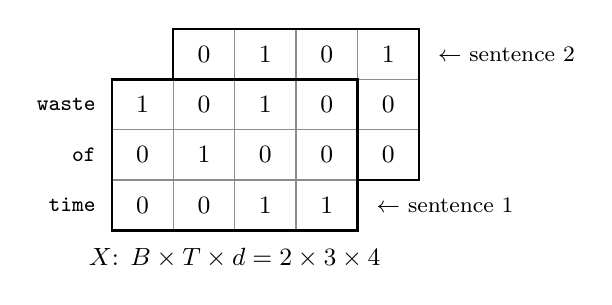
\begin{tikzpicture}
\fill[white] (0.780,0.640) rectangle (3.900,-1.279);
\draw[black!45, fill=white] (0.780,0.640) rectangle (1.560,0.000);
\node[font=\small, text=black] at (1.170,0.320) {$0$};
\draw[black!45, fill=white] (1.560,0.640) rectangle (2.340,0.000);
\node[font=\small, text=black] at (1.950,0.320) {$1$};
\draw[black!45, fill=white] (2.340,0.640) rectangle (3.120,0.000);
\node[font=\small, text=black] at (2.730,0.320) {$0$};
\draw[black!45, fill=white] (3.120,0.640) rectangle (3.900,0.000);
\node[font=\small, text=black] at (3.510,0.320) {$1$};
\draw[black!45, fill=white] (0.780,0.000) rectangle (1.560,-0.640);
\node[font=\small, text=black] at (1.170,-0.320) {$1$};
\draw[black!45, fill=white] (1.560,0.000) rectangle (2.340,-0.640);
\node[font=\small, text=black] at (1.950,-0.320) {$0$};
\draw[black!45, fill=white] (2.340,0.000) rectangle (3.120,-0.640);
\node[font=\small, text=black] at (2.730,-0.320) {$0$};
\draw[black!45, fill=white] (3.120,0.000) rectangle (3.900,-0.640);
\node[font=\small, text=black] at (3.510,-0.320) {$0$};
\draw[black!45, fill=white] (0.780,-0.640) rectangle (1.560,-1.279);
\node[font=\small, text=black] at (1.170,-0.959) {$0$};
\draw[black!45, fill=white] (1.560,-0.640) rectangle (2.340,-1.279);
\node[font=\small, text=black] at (1.950,-0.959) {$0$};
\draw[black!45, fill=white] (2.340,-0.640) rectangle (3.120,-1.279);
\node[font=\small, text=black] at (2.730,-0.959) {$1$};
\draw[black!45, fill=white] (3.120,-0.640) rectangle (3.900,-1.279);
\node[font=\small, text=black] at (3.510,-0.959) {$0$};
\draw[line width=0.9pt] (0.780,0.640) rectangle (3.900,-1.279);
\node[anchor=west, font=\footnotesize] at (4.020,0.320) {$\leftarrow$ sentence 2};
\fill[white] (0.000,0.000) rectangle (3.120,-1.919);
\draw[black!45, fill=white] (0.000,0.000) rectangle (0.780,-0.640);
\node[font=\small, text=black] at (0.390,-0.320) {$1$};
\draw[black!45, fill=white] (0.780,0.000) rectangle (1.560,-0.640);
\node[font=\small, text=black] at (1.170,-0.320) {$0$};
\draw[black!45, fill=white] (1.560,0.000) rectangle (2.340,-0.640);
\node[font=\small, text=black] at (1.950,-0.320) {$1$};
\draw[black!45, fill=white] (2.340,0.000) rectangle (3.120,-0.640);
\node[font=\small, text=black] at (2.730,-0.320) {$0$};
\draw[black!45, fill=white] (0.000,-0.640) rectangle (0.780,-1.279);
\node[font=\small, text=black] at (0.390,-0.959) {$0$};
\draw[black!45, fill=white] (0.780,-0.640) rectangle (1.560,-1.279);
\node[font=\small, text=black] at (1.170,-0.959) {$1$};
\draw[black!45, fill=white] (1.560,-0.640) rectangle (2.340,-1.279);
\node[font=\small, text=black] at (1.950,-0.959) {$0$};
\draw[black!45, fill=white] (2.340,-0.640) rectangle (3.120,-1.279);
\node[font=\small, text=black] at (2.730,-0.959) {$0$};
\draw[black!45, fill=white] (0.000,-1.279) rectangle (0.780,-1.919);
\node[font=\small, text=black] at (0.390,-1.599) {$0$};
\draw[black!45, fill=white] (0.780,-1.279) rectangle (1.560,-1.919);
\node[font=\small, text=black] at (1.170,-1.599) {$0$};
\draw[black!45, fill=white] (1.560,-1.279) rectangle (2.340,-1.919);
\node[font=\small, text=black] at (1.950,-1.599) {$1$};
\draw[black!45, fill=white] (2.340,-1.279) rectangle (3.120,-1.919);
\node[font=\small, text=black] at (2.730,-1.599) {$1$};
\draw[line width=0.9pt] (0.000,0.000) rectangle (3.120,-1.919);
\node[anchor=east, font=\footnotesize\ttfamily] at (-0.080,-0.320) {waste};
\node[anchor=east, font=\footnotesize\ttfamily] at (-0.080,-0.959) {of};
\node[anchor=east, font=\footnotesize\ttfamily] at (-0.080,-1.599) {time};
\node[anchor=west, font=\footnotesize] at (3.240,-1.599) {$\leftarrow$ sentence 1};
\node[anchor=north, font=\small] at (1.560,-2.019) {$X$: $B\times T\times d = 2\times3\times4$};
\end{tikzpicture}
\end{center}

\begin{wrongidea}{2.4}
``Token 1 and token 2 are close, so their meanings are close.'' The number only says which row to open.
In our table, row 1 (\tok{of}) and row 2 (\tok{time}) are at right angles: their dot product is 0. Meaning
lives in the arrows, never in the locker numbers.
\end{wrongidea}

\begin{wrongidea}{2.5}
``The vector of a word changes with the sentence.'' It is tempting because a word's meaning does
change with the sentence. But the row for \tok{time} is the same in \emph{time flies} and in
\emph{waste of time}. What changes with context is the arrow \emph{after} attention has mixed in the other
tokens (Chapter 3). The table gives every token the same starting point; the layers do the rest.
\end{wrongidea}

\begin{checkq}
What does multiplying the one-hot row for \tok{useful} (a 1 in position 5) by $E$ give?
\begin{options}
\item $(0,0,1,0)$, row 5 of the table.
\item $5\times(1,1,1,1)$, because the 1 sits in position 5.
\item The sum of all twelve rows, since every row is multiplied.
\item A number between 0 and 1 saying how useful the word is.
\end{options}
\end{checkq}

\Summary{a token number opens one row of the embedding table, and that row, an arrow of $d$ numbers, is
where the model's knowledge about the token starts.}

%---------------------------------------------------------------------
\subsection*{2.5\quad Where do good arrows come from?}

Our toy arrows were chosen by hand. Requirement 1 of Chapter 1 asks for more: \emph{similar words must
get similar arrows}, so that what is learned about one transfers to the other. How could a machine know
that \tok{money} and \tok{amount} are alike, if nobody tells it?

\Picture You learn what kind of person someone is by talking with them and seeing who they spend time
with. A word is the same. The linguist J. R. Firth put it in 1957: ``You shall know a word by the company
it keeps.'' Words that keep the same company are used for the same things.

\paragraph{The numbers.} Let us build arrows from company alone. We took the \nTwoWvVocab\ most frequent
words of parts 1--8 and counted, for each pair of words, how often they appear within \nTwoWvWin\ words
of each other. Then we kept only the pairs that occur together more often than chance would predict, and
compressed each word's row of counts to $\nTwoWvDim$ numbers (the method is in \texttt{code/ch2\_bpe.py};
Levy and Goldberg, 2014, showed it is closely related to the popular \emph{word2vec} of Mikolov and
colleagues, 2013). Nobody told the program anything about meaning. Here are the nearest arrows it found,
with their cosine (the agreement $\cos\theta$ from Chapter 3):

\begin{center}
\small
\begin{tabular}{@{}l l@{}}
\toprule
word & nearest words in parts 1--8 (cosine)\\
\midrule
\tok{money} & \nTwoNNMoney\\
\tok{model} & \nTwoNNModel\\
\tok{question} & \nTwoNNQuestion\\
\tok{time} & \nTwoNNTime\\
\bottomrule
\end{tabular}
\end{center}

\tok{money} lands next to \tok{amount} and \tok{costs}; \tok{model} next to \tok{models}, \tok{tuned} and
\tok{quen} (how the corpus spells Qwen). Now look at \tok{time}. Its neighbours are \tok{same},
\tok{at}, \tok{point}: in these talks, ``time'' mostly lives in \emph{at the same time} and \emph{at this
point in time}. The arrows learn how a word is \emph{used in this text}, not what a dictionary says. The
cosine between \tok{time} and \tok{money} is \nTwoCosTimeMoney, while any two different one-hot rows
have cosine \nTwoOneHotCos: the counting notebook of Chapter 1 had no way to see any resemblance at all.

\Exactly An embedding is a map from tokens to $\mathbb{R}^d$ chosen so that the geometry carries
information: tokens used in similar contexts get a small angle between them. In this section the map came
from counting. In a transformer the table $E$ is learned by the next-token game itself (Chapter 8): if
two tokens tend to be followed by the same words, the nudges that improve one also improve the other, and
their rows drift together.

\begin{breaks}
The ``company'' picture says nothing about \emph{which} company. \tok{good} and \tok{bad} keep almost the
same company (``a \underline{\ \ } answer'', ``very \underline{\ \ }''), so counting puts them close
together even though they are opposites. A model that needs to tell them apart has to learn it from the
next-word game, where they \emph{are} followed by different words.
\end{breaks}

\begin{wrongidea}{2.6}
``Each of the 64 numbers means something you can name, like sentiment.'' It is tempting because in a churn model,
each clue had a name: number of logins, days since last purchase. Embedding coordinates do not. The
compression is free to spread one idea over many coordinates and to pack many ideas into one. Directions
can carry meaning; single coordinates rarely do.
\end{wrongidea}

\begin{checkq}
Our arrows put \tok{time} near \tok{same} and \tok{point}. What does that tell you?
\begin{options}
\item The method failed, because \tok{time} should be next to \tok{day}.
\item In these talks, \tok{time} is mostly used in phrases like \emph{at the same time}, and the
arrows record usage.
\item Someone labelled \tok{time} and \tok{same} as synonyms.
\item The fourth coordinate of each arrow stores the word's meaning, and they share it.
\end{options}
\end{checkq}

\Summary{arrows built only from which words appear together already place similar words close together,
and a transformer learns its own arrows the same way, from the next-word game.}

%---------------------------------------------------------------------
\subsection*{2.6\quad Requirement 1 is met. What is still missing?}

We now have what Chapter 1 asked for: a way to read any text (byte-pair encoding) and a starting arrow for
every piece, with similar pieces near each other. But look again at \S2.4: the row for \tok{time} is the
same in every sentence. A support reply to \emph{waste of time} and a calendar reminder about \emph{on time}
start from the same arrow. The arrow has to change once the token has seen its neighbours. That is
exactly the job of attention, and it is where Chapter 3 begins.

\begin{principle}{give frequent things a short name and rare things a way to be spelled}
Byte-pair encoding is a compression rule: short codes for what is common, a guaranteed fallback for
everything else. The same rule appears in good systems everywhere: a cache keeps hot items close and goes
to disk for the rest; an agent's tool list gives common actions a named tool and leaves a general
fallback (``run this command'') for the rest. And the embedding idea, \emph{put similar things close
together and search by angle}, is the whole basis of retrieval in an agent's memory system: a memory is
stored as an arrow, and recall means finding the stored arrows with the smallest angle to the question.
\end{principle}

\begin{lookingback}
(a) Chapter 1 measured that \cUnseenThree\% of three-word sequences in part 9 were never seen before.
Does byte-pair encoding fix that problem? (b) Which of the four requirements from Chapter 1 does this
chapter meet? (c) In Chapter 3, which matrix was the first to act on the arrows that come out of the
embedding table?
\end{lookingback}

%---------------------------------------------------------------------
\subsection*{Exercises}

\begin{exercise}
Run one step of byte-pair encoding by hand on the text \tok{waste waste wasted time} (each word followed
by \tok{\_}). Which pair, or pairs, are most frequent, and how many times does each appear? What must a real
tokenizer do when there is a tie?
\end{exercise}

\begin{exercise}
Compute the cosine between the toy arrows of \tok{waste} and \tok{time}. Then compute it between the
one-hot rows of the same two tokens. Which one could ever tell you the words are related?
\end{exercise}

\begin{exercise}
A model has $V=50{,}000$ tokens and $d=768$. How many numbers are in its embedding table? If you double
the vocabulary, what happens to the table, and what (from \S2.2) do you expect to happen to the length of a
typical sentence?
\end{exercise}

\begin{exercise}
Explain to a friend who has never programmed why a model with a byte-level vocabulary can read a word it has
never seen, but may still not understand it. Use the locker picture and say where it stops working.
\end{exercise}

%---------------------------------------------------------------------
\subsection*{Answers to Chapter 2}

\noindent\textbf{Check yourself 2.1.} (a). Each new product name has no row. (b) is wrong: letters never run
out; long names cost length, not failure. (c) reflects M2.1: the model does not read like a person, it only
gets token numbers. (d) confuses length with novelty.

\noindent\textbf{Check yourself 2.2.} (b). Merges follow frequency in the training text. (a) reflects a
belief that the tokenizer judges meaning; it only counts. (c): byte-pair pieces need not be syllables
(\tok{as}, \tok{te\_}). (d): length matters only through frequency; a long common word can be one token.

\noindent\textbf{Check yourself 2.3.} (a). The one-hot row selects row 5. (b) treats the token number as a
quantity (M2.4). (c) forgets that eleven of the twelve multipliers are zero. (d) treats the arrow's numbers
as nameable scores (M2.6).

\noindent\textbf{Check yourself 2.4.} (b). The arrows record how a word is used here. (a) expects
dictionary meaning; (c) is M2.7, since nobody labelled anything; (d) is M2.6.

\noindent\textbf{Looking back.} (a) No. Byte-pair encoding makes every \emph{word} readable, but a counting
model still needs to have seen the same \emph{sequence}; that problem is solved by arrows plus attention.
(b) Requirement 1, similarity. (c) $W_Q$, $W_K$ and $W_V$ act on the arrows.

\noindent\textbf{Exercise 2.1.} \nTwoExTies\ pairs tie, each seen \nTwoExTopCount\ times: \nTwoExTiePairs.
A tokenizer needs a fixed tie-breaking rule (for example, alphabetical order) so that the same text always
gives the same tokens.

\noindent\textbf{Exercise 2.2.} The toy arrows $(1,0,1,0)$ and $(0,0,1,1)$ have dot product 1 and lengths
$\sqrt2$ each, so the cosine is $1/2 = \nTwoCosToyWasteTime$. The one-hot rows have cosine \nTwoOneHotCos,
as any two different one-hot rows do. Only the arrows can express a relation.

\noindent\textbf{Exercise 2.3.} $50{,}000\times768 = \nTwoExThreeTable$ numbers. Doubling the vocabulary doubles
the table. Sentences get shorter, since more letter-groups have their own token, but by less each time:
the curve in \S2.3 flattens.

\noindent\textbf{Exercise 2.4.} Any word can be written as bytes, so it always gets a list of lockers to
open. But each locker holds the arrow of a \emph{piece}, and the meaning of the whole word has to be
assembled by later layers from the pieces and the context. The locker picture stops working there:
lockers are independent, while a word's meaning depends on its neighbours.

\paragraph{What you now know.}
\begin{itemize}
\item Why neither whole words nor single letters work, with the numbers that show it.
\item How byte-pair encoding builds a vocabulary by merging the most frequent pair, again and again.
\item That an embedding is one row of a table, fetched by a one-hot row times a matrix.
\item That token numbers carry no meaning, and that arrows built from word company place similar words
close together.
\end{itemize}
